%%%%%%%%%%%%%%%%%%%%%%%%%%%%%%%%%%%%%%%%%%%%%%%%%%%%%%%%%%%%%%%%%%%
%                                                                 %
%  GEANT manual in LaTeX form                              %
%                                                                 %
%  Michel Goossens (for translation into LaTeX)                   %
%  Version 1.00                                                   %
%  Last Mod. Jan 24 1991  1300   MG + IB                          %
%                                                                 %
%%%%%%%%%%%%%%%%%%%%%%%%%%%%%%%%%%%%%%%%%%%%%%%%%%%%%%%%%%%%%%%%%%%
\Origin{R.Brun}
\Submitted{01.11.83}      \Revised{14.12.93}
\Version{Geant 3.16}\Routid{KINE199}
\Makehead{The data structures JVERTX and JKINE}

\begin{figure}[hbt]
     \centering
     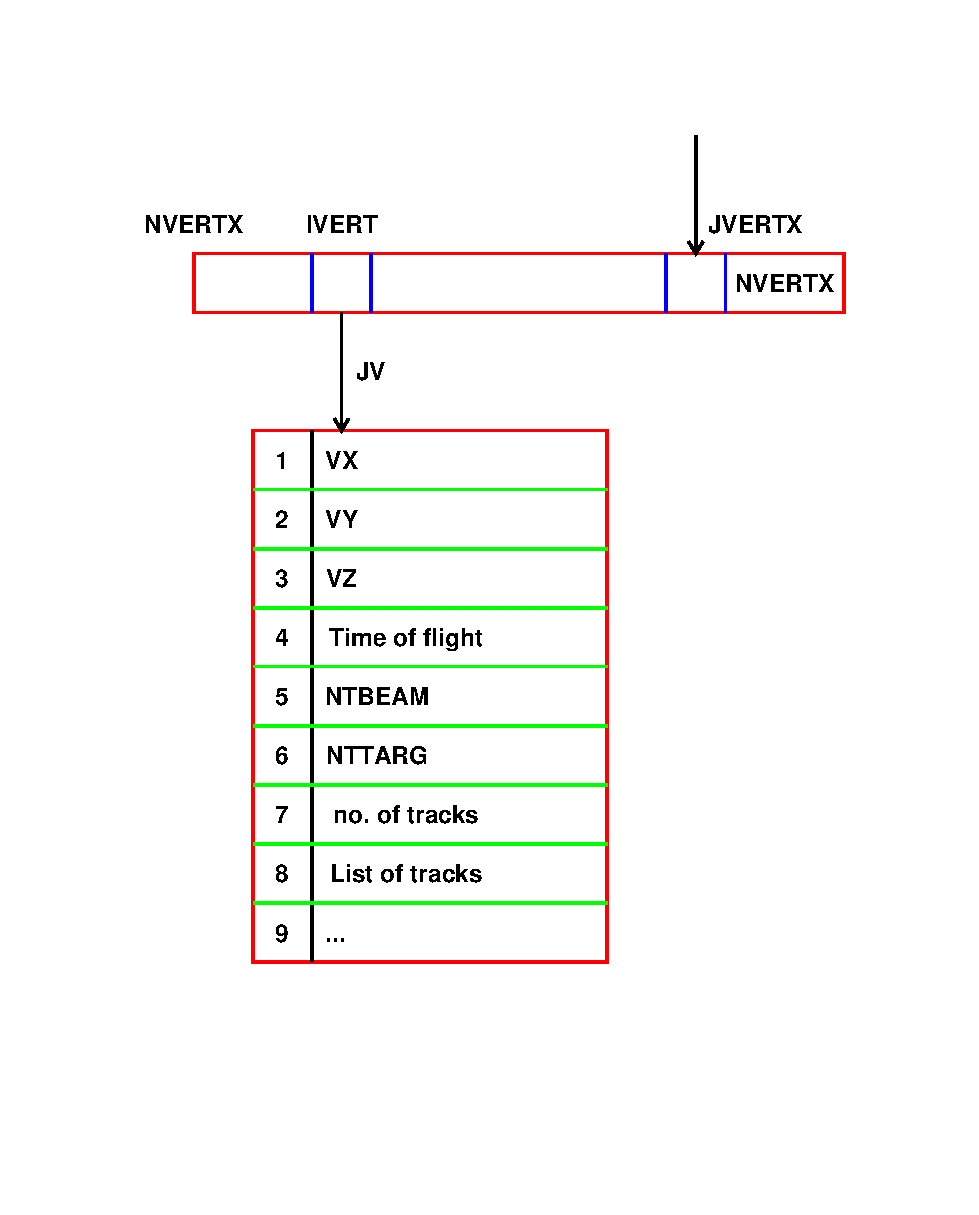
\epsfig{file=eps/kine199-1.eps,width=14cm}
     \caption{Layout of the {\tt JVERTX} data structure}
     \label{fg:kine199-1}
\end{figure}

\begin{DLtt}{MMMM}
\item[JV]= LQ(JVERTX-IVERT) pointer to the bank of vertex {\tt IVERT}.
\item[JVU]= {\tt LQ(JV-1)} pointer to the user part of the bank.
\end{DLtt}

The {\tt JVERTX} banks are filled by the routine \Rind{GSVERT} and \Rind{GSVERU}.
Vertex parameters can be retrieved by the routine \Rind{GFVERT} and printed
by the routine \Rind{GPVERT}.
 
\clearpage

\begin{figure}[hbt]
     \centering
     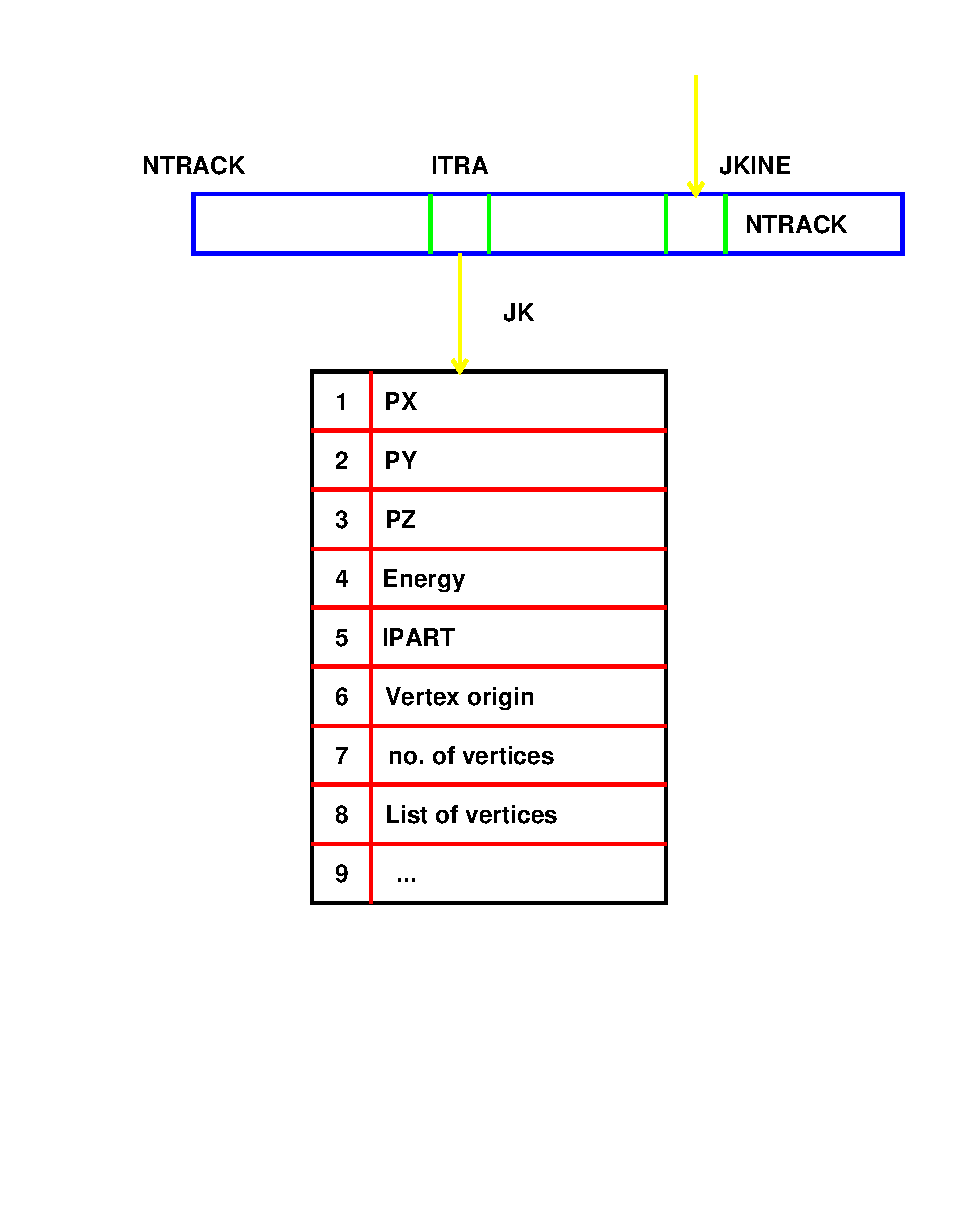
\epsfig{file=eps/kine199-2.eps,width=14cm}
     \caption{Layout of the {\tt JKINE} data structure}
     \label{fg:kine199-2}
\end{figure}

 
\begin{DLtt}{MMMM}
\item[JK]= {\tt LQ(JKINE-ITRA)} pointer to the bank of track {\tt ITRA}.
\item[JKU]= {\tt LQ(JK-1)} pointer to the user part of the bank.
\end{DLtt}
 
The {\tt JKINE} banks are filled by the routine \Rind{GSKINE} and \Rind{GSKINU}.
Track parameters can be retrieved by the routine \Rind{GFKINE} and printed
by the routine \Rind{GPKINE}.
